\documentclass[final]{beamer}

\usetheme{RJH}
\setbeamertemplate{bibliography item}[text]
\usepackage[orientation=landscape,size=a0,scale=1.4,debug]{beamerposter}
\usepackage[absolute,overlay]{textpos}
\setlength{\TPHorizModule}{1cm}
\setlength{\TPVertModule}{1cm}

\title{Fast Point Cloud Registration using Gaussian Processes}
\author{Ben Eckart\inst{1}, Seth Flaxman\inst{2,3}, Antonio Juarez\inst{2}}
\footer{Carnegie Mellon University: 10-725 Optimization Final Project}
\institute{\inst{1} Robotics Institute\and %
                      \inst{2} Machine Learning Department\and %
                      \int{3} Heinz College}

\date{}

\begin{document}
\bibliographystyle{plain}
\begin{frame}{} 

\begin{textblock}{27}(1.5,5)
\begin{block}{Motivation: Automatic Mapping of the World}
\begin{figure}
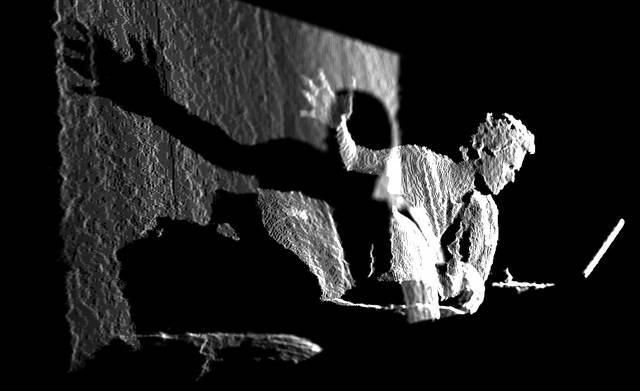
\includegraphics[width=10in]{kyle_kinect.jpg}
\caption{Kinect photo by Kyle McDonald (CC-BY-SA-NC)}
\end{figure}

3D range sensors like Velodyne and Kinect generate massive amounts of data, on the order of
{\bf one million data points per second}.

Standard optimization algorithms for real-time perception aren't adequate.
\end{block}

\begin{block}{Related Work: The Registration Problem}

{\bf Iterative Closest Point (ICP) algorithm \cite{besl_method_1992}} 
\begin{figure}
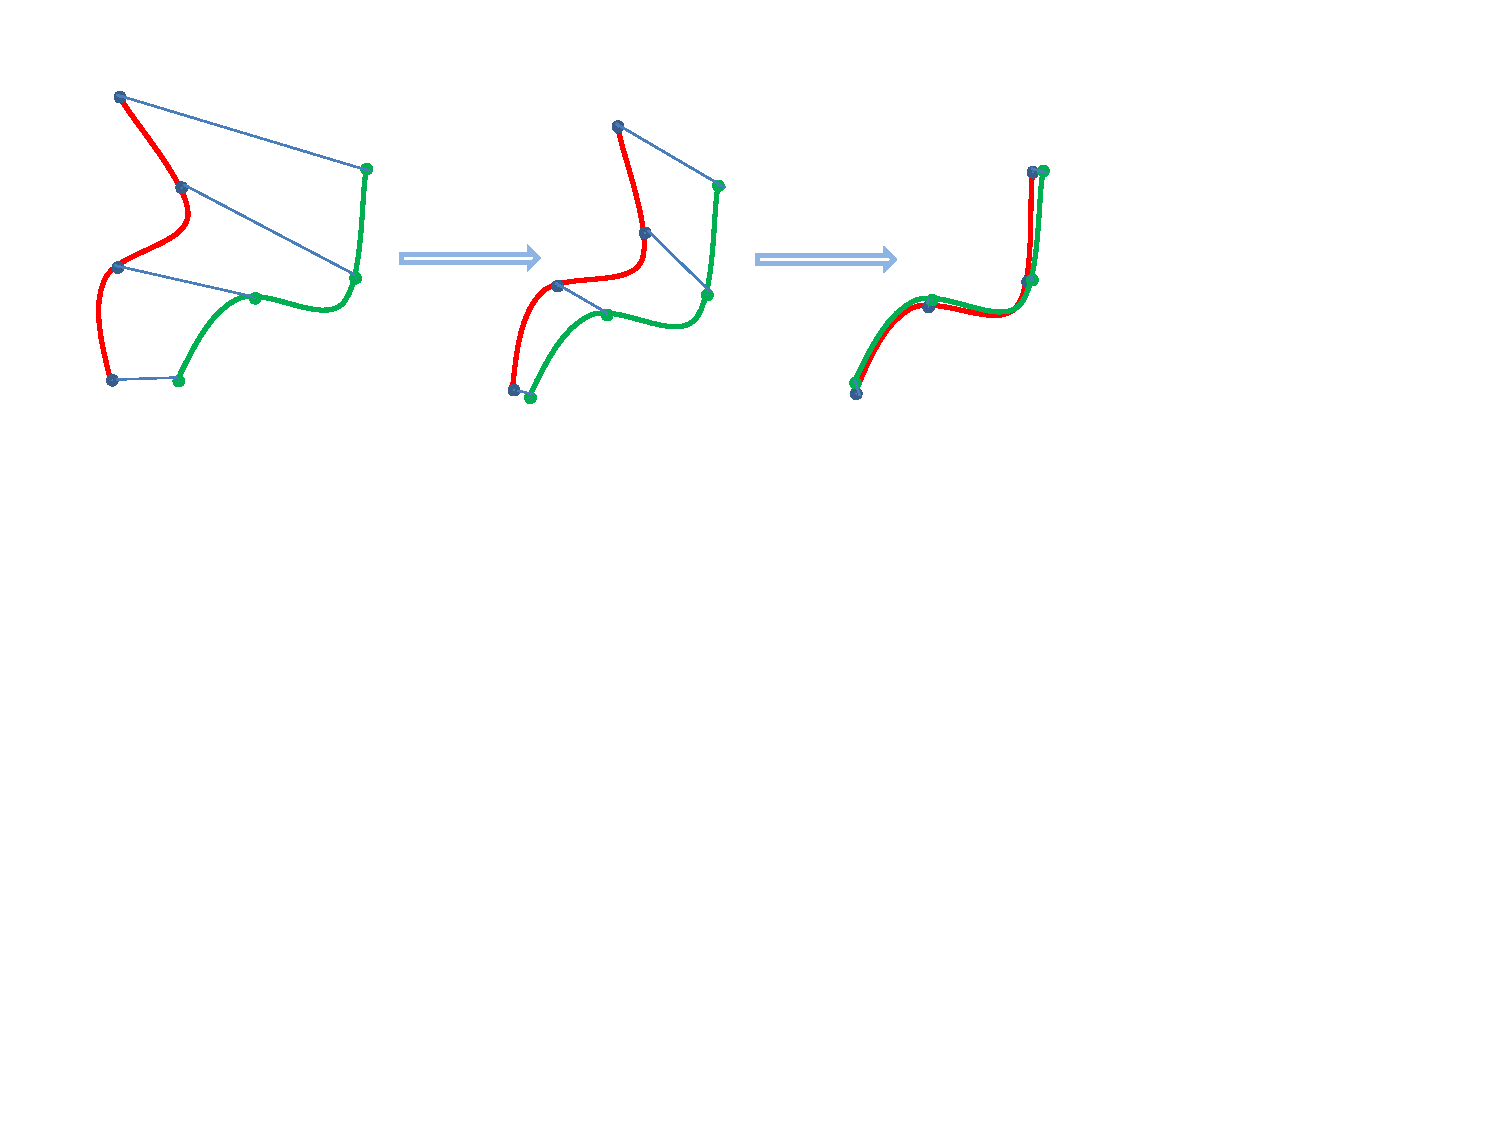
\includegraphics[width=10in]{ICP.pdf}
\end{figure}

{\bf Gaussian Mixture Models (GMM) \cite{jian_robust_5555}}
\begin{figure}
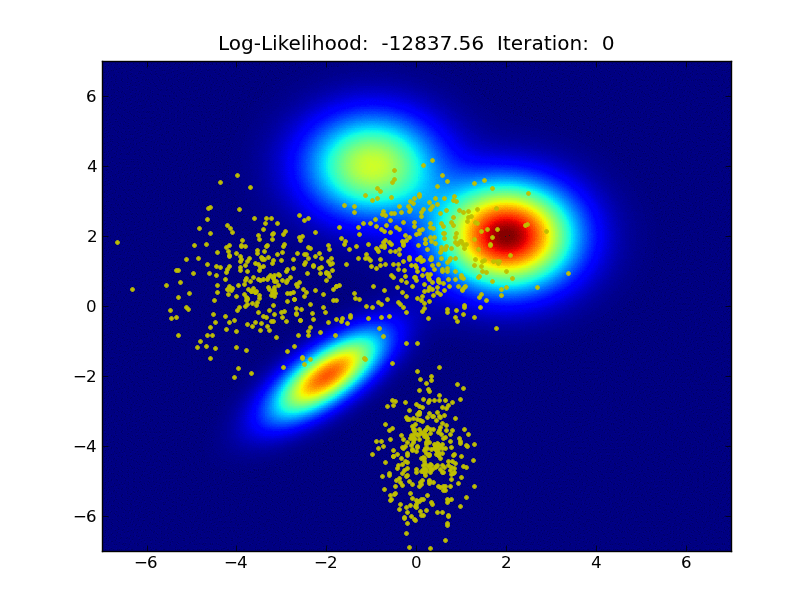
\includegraphics[width=10in]{register2D.png}
\end{figure}

\end{block}

\begin{block}{Affiliations}
1. Robotics Institute \\
2. Machine Learning Department \\
3. Heinz College
\end{block}
\end{textblock}

\begin{textblock}{27.5}(30.8,5)
\begin{block}{Gaussian Processes (GPs)}
A distribution over functions, fully specified by a mean and a covariance:
$f \sim \mathcal{GP}(m,k)$ \cite{rasmussen2006gaussian}. Given a set of points $(x,y,z)$ and a new point $(x_*,y_*)$ for which we want to predict $z_*$, 
distribution is simply {\bf multivariate Gaussian} with:
$$\mu = K_* (K + \sigma^2 I)^{-1}z$$
$$\Sigma = K_{**} - K_* (K + \sigma^2 I)^{-1} K_*^T$$
\end{block}

\begin{block}{3D Model}
{\bf Dataset}: A cloud of 3-D points

{\bf Representation}: An elevation map (x,y) $\rightarrow$ z

The Gaussian Process induces a probability distribution on the elevation of every (x,y)

\begin{center}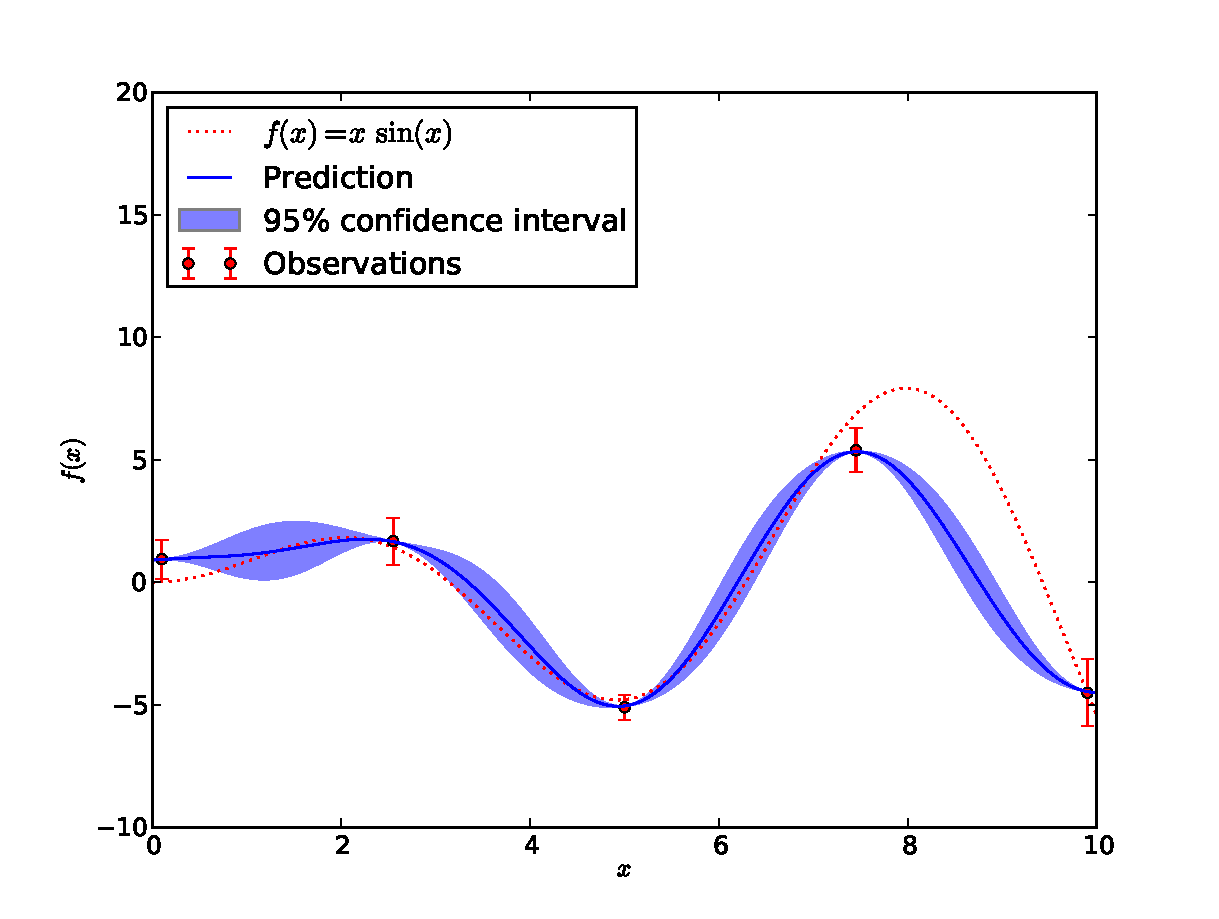
\includegraphics[width=5.0in]{1DGaussianProcess.pdf}\end{center}
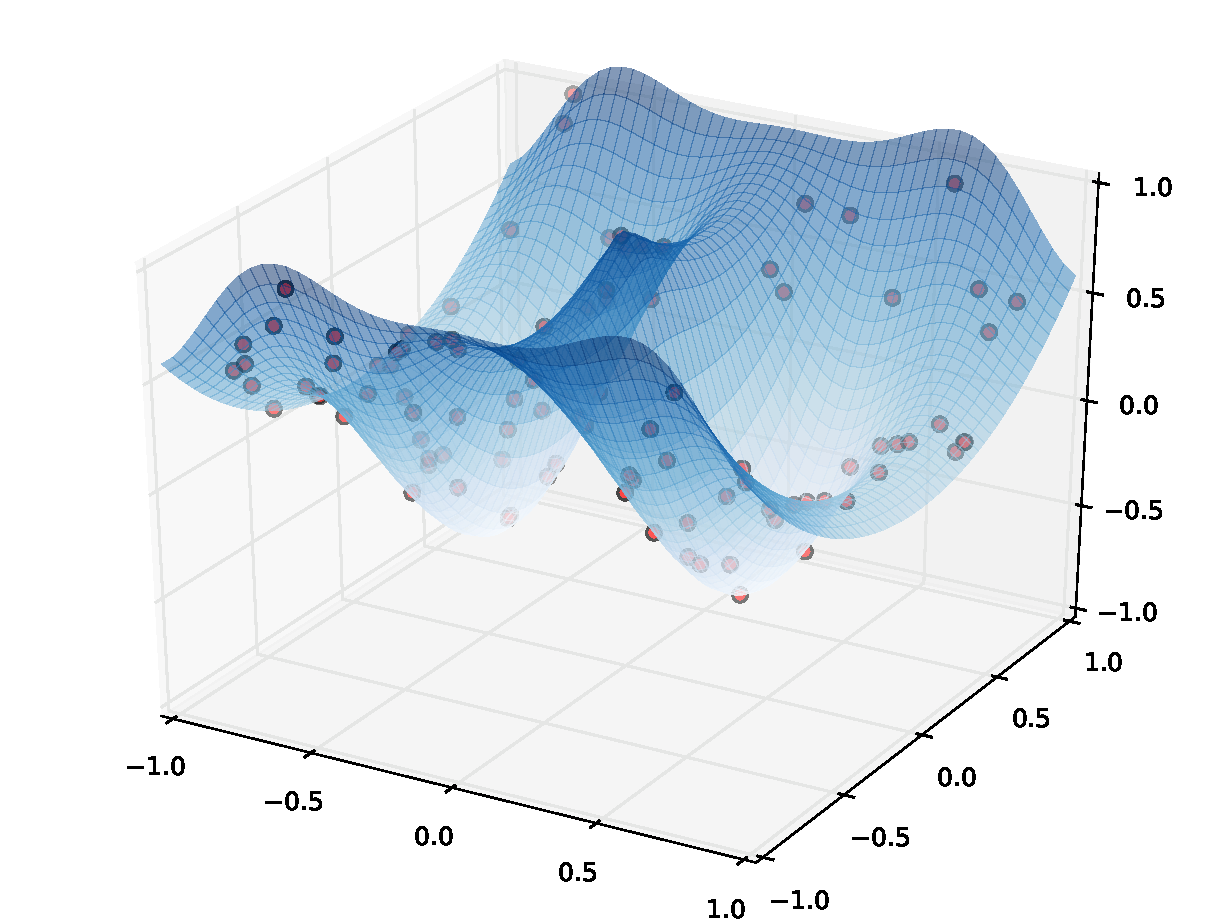
\includegraphics[width=5.0in]{2DGaussianProcess1.pdf}
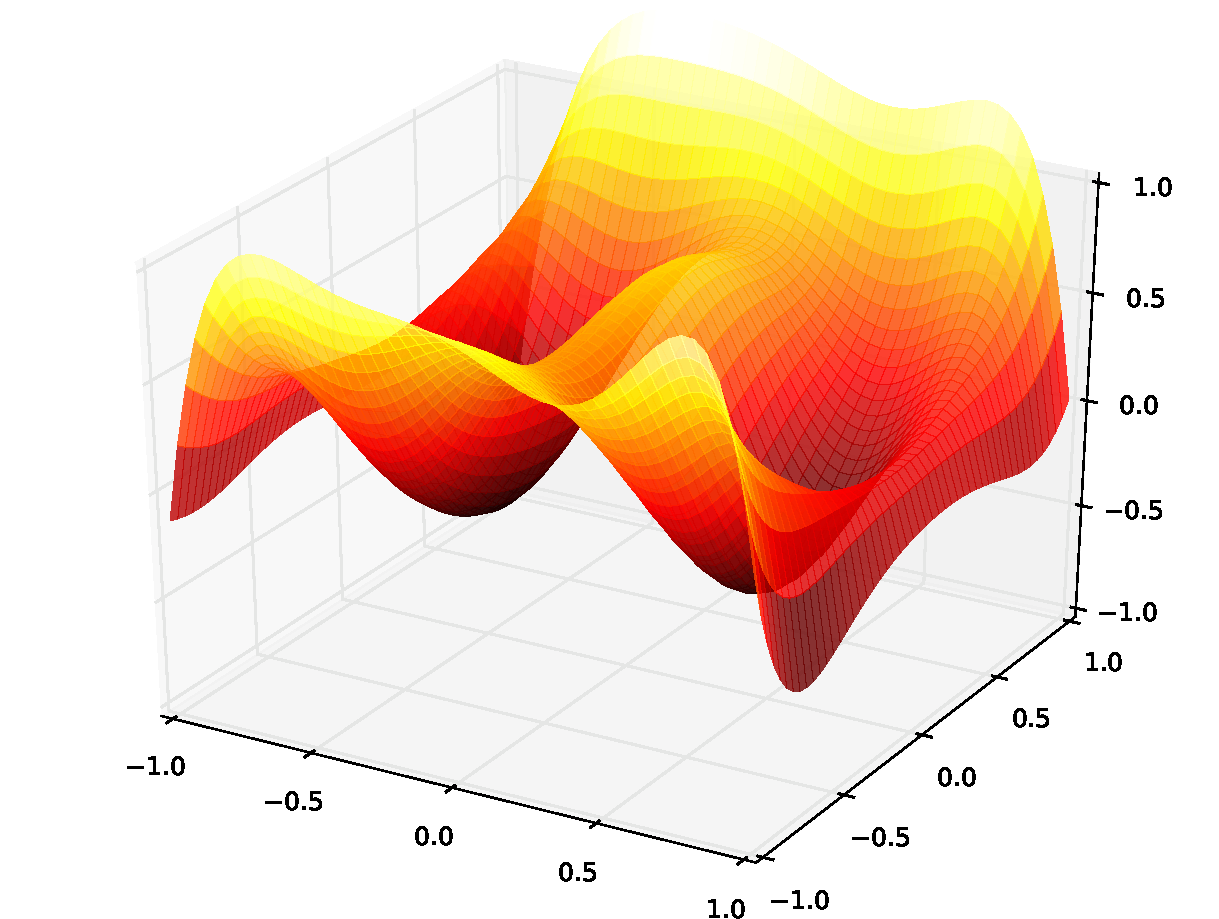
\includegraphics[width=5.0in]{2DGaussianProcess2.pdf}

\end{block}

\begin{block}{Estimating the Transformation}
Given two consecutive frames of 3D cloud datasets, we aim to find the most likely rigid transformation that converted the first into the second.

\textbf{Input:} Two consecutive 3D datasets

\textbf{Output:} The most likely rigid transformation from one scene to the other.
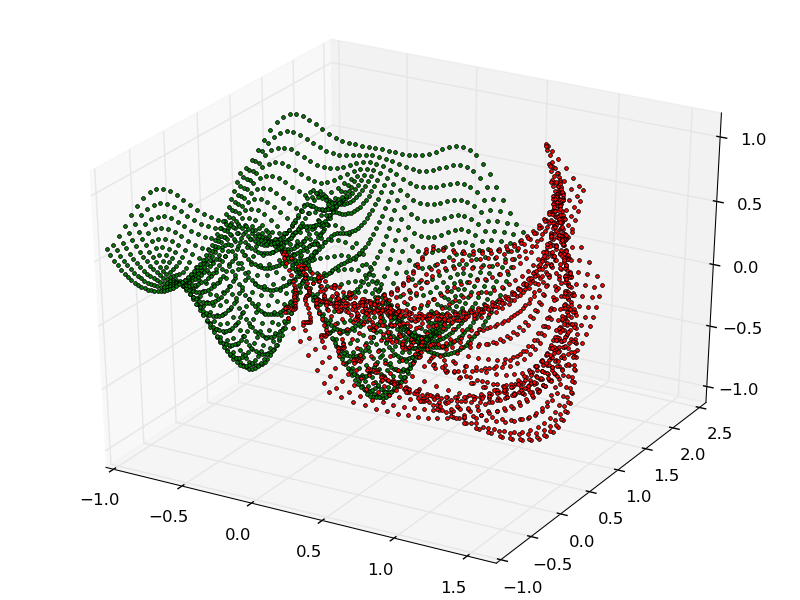
\includegraphics[width=10in]{3DWorldModel.png}
\end{block}

\end{textblock}

\begin{textblock}{27}(61,5)




\begin{block}{Registration as an Optimization Problem}
Given a scene and a set of new points, find a rigid transformation $T = [T_x,T_y,T_z,q]$ of the new points 
that maximizes their likelihood in the original scene, which is fit with a GP:
$$\min -\log\mathcal{L}(T|x,y,z,x_*,y_*,z_*) =$$
$$ \min \log|\Sigma| + (T(z_*) - \mu)^T \Sigma^{-1} (T(z_*) - \mu)$$
(where $T([x,y,z]^T) = R(q)[x,y,z]^T + [T_x,T_y,T_z]^T$).

\end{block}


\begin{block}{Parameter Space}
Our parameter search space (parameters of T) is 7-D.
\vspace{-.1in}
\begin{figure}
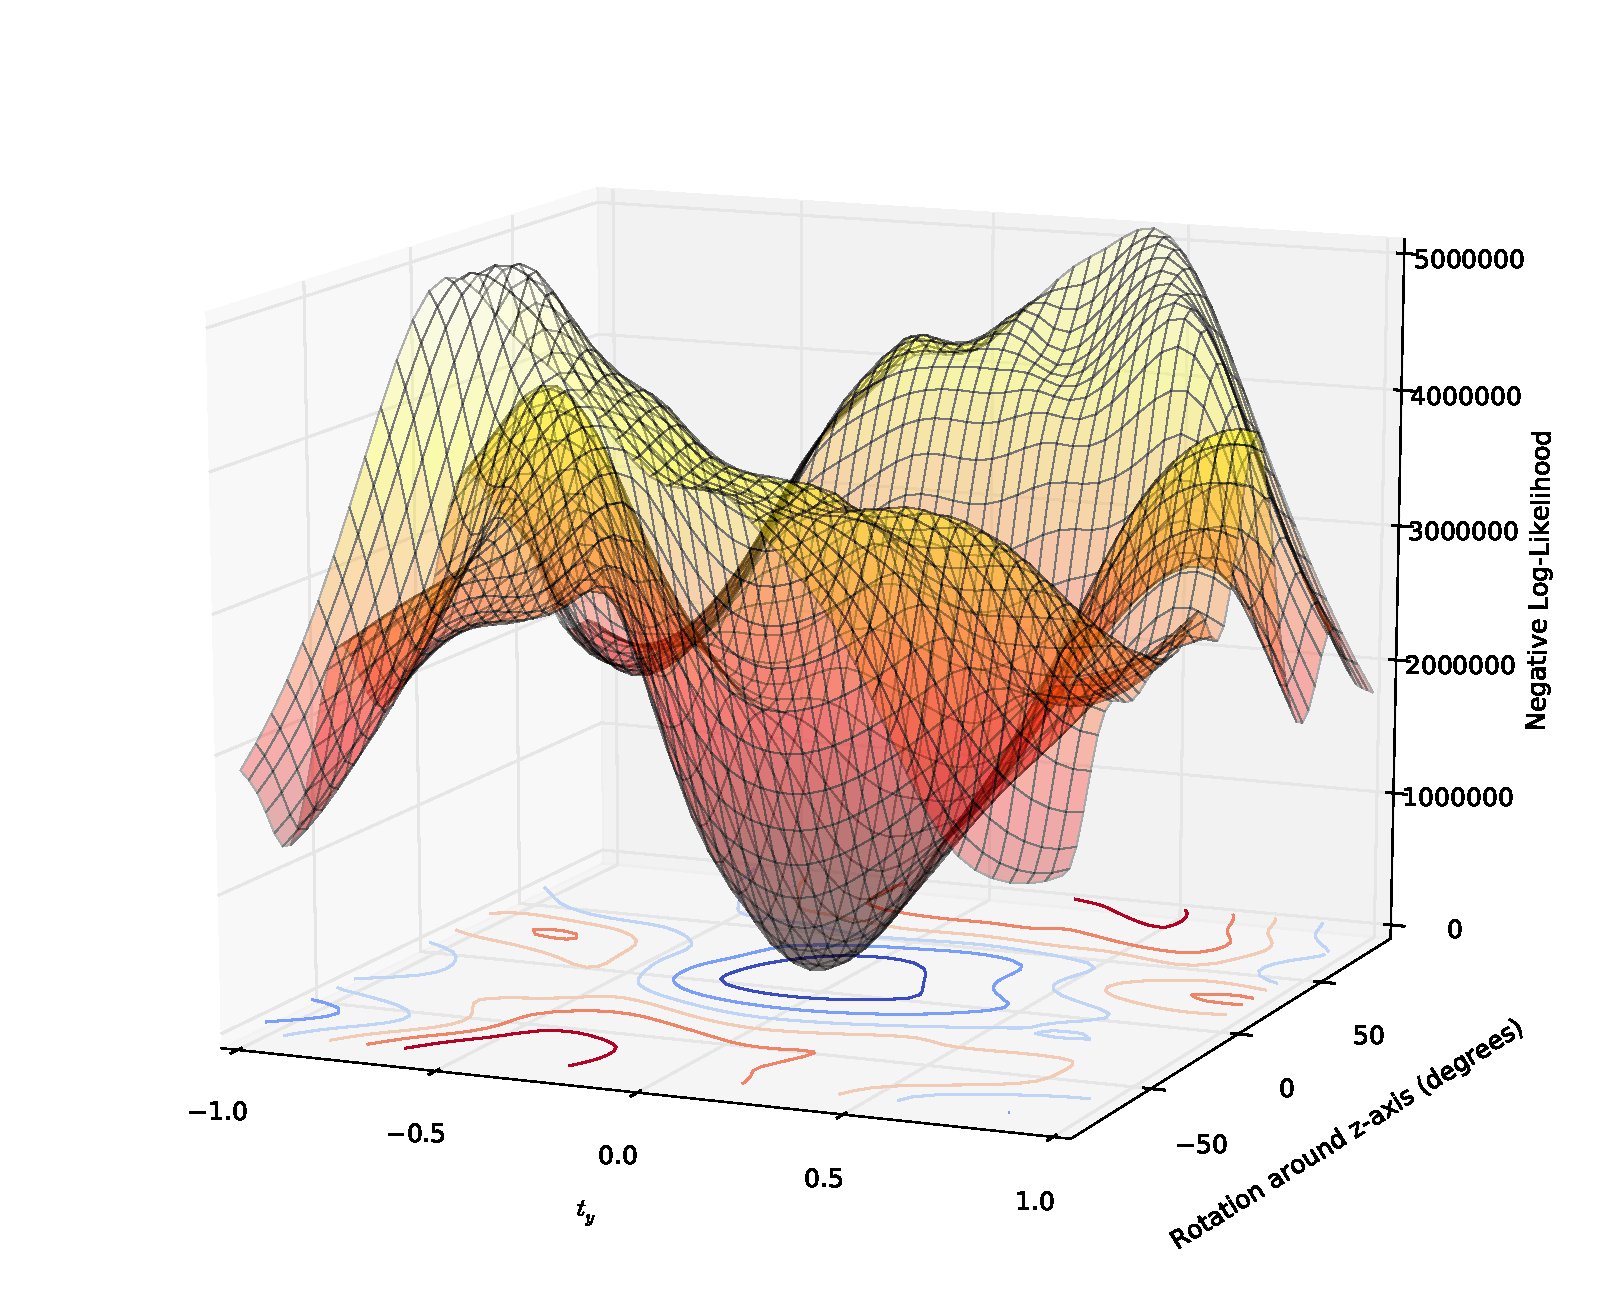
\includegraphics[width=10in]{LLmap3.pdf}
\caption{2-D Projection of the likelihood}
\end{figure}
Note that this problem is not convex; the minimum we care about may {\bf not} be the global minimum. 
\end{block}

\begin{block}{Gradient Descent}
Partial derivatives must be found with respect to the 7 parameters of $T$. Each can be written in closed form,
using {\bf matrix} and {\bf quaternion} calculus. Numerical stability and speed relies on the {\bf Cholesky} decomposition. {\bf Backtracking line search} and {\bf acceleration} are natural extensions.
\end{block}


\begin{block}{References}
{
\footnotesize
\bibliographystyle{plain}
% argument is your BibTeX string definitions and bibliography database(s)
\bibliography{./full}
}
\end{block}


\end{textblock}
\begin{textblock}{27}(91,5)

\begin{block}{Experiments and Comparisons with ICP}
To compare our method with ICP, we generated artificial test data from a smooth distribution.

%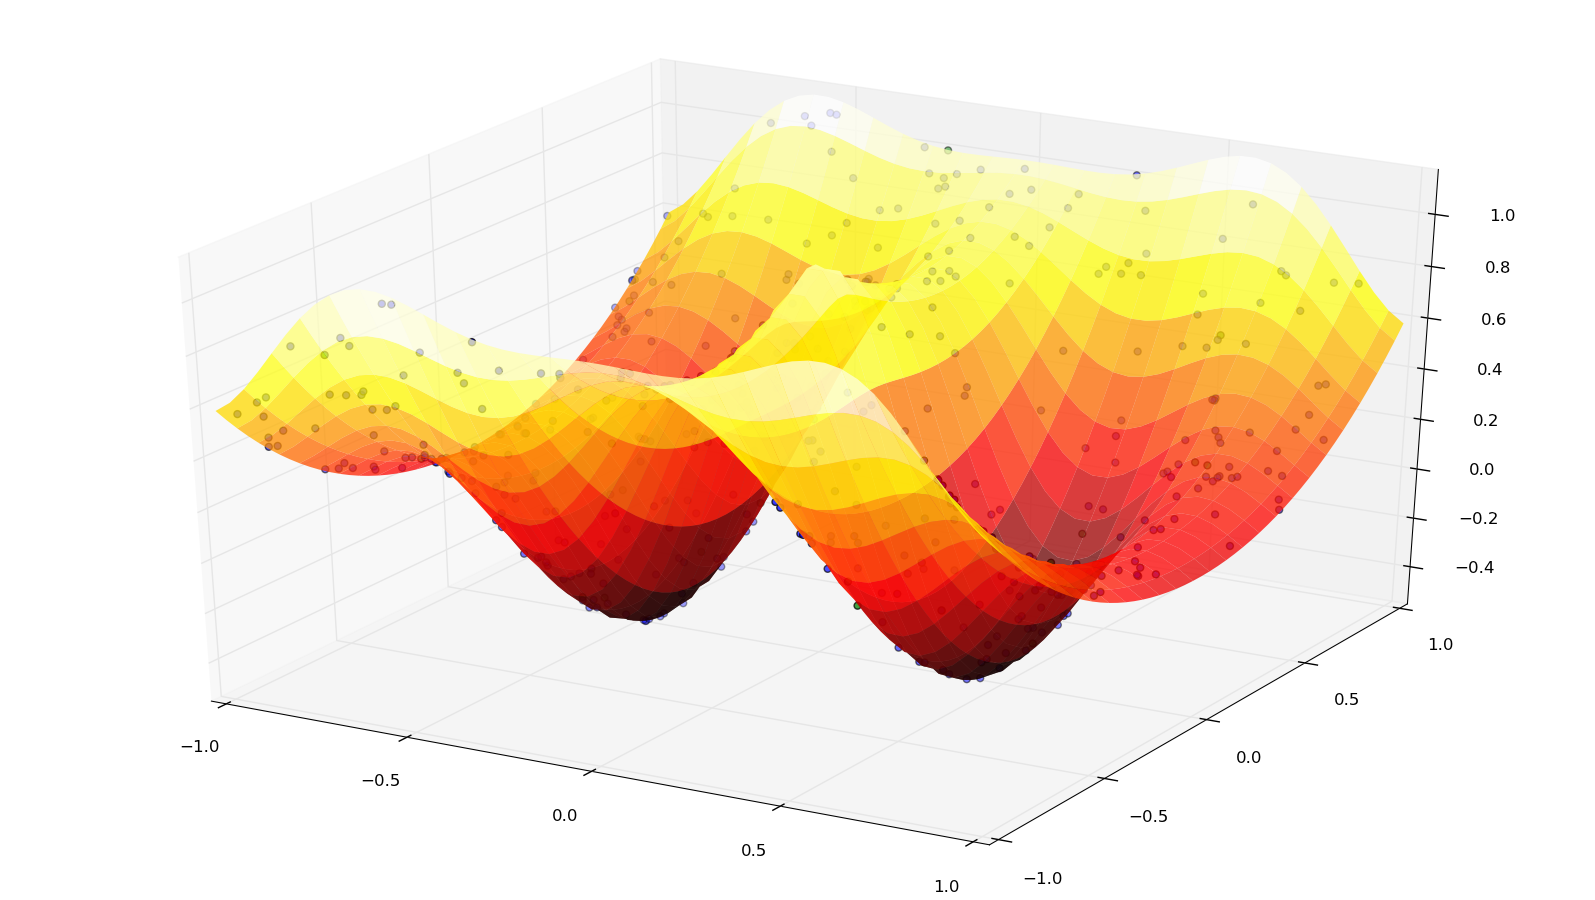
\includegraphics[width=5in]{DistributionPlusPoints.png}
%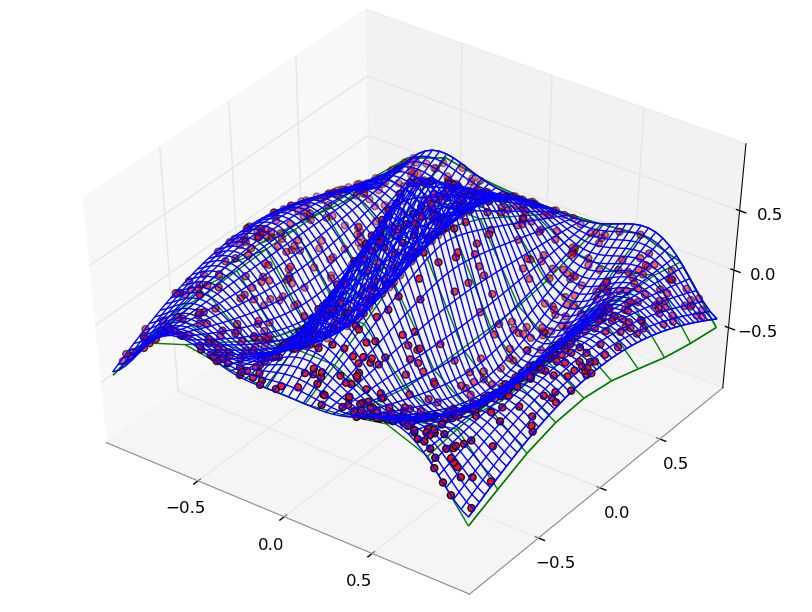
\includegraphics[width=5in]{Reconstruction.png}

%\begin{block}{Results}
%\begin{figure}
%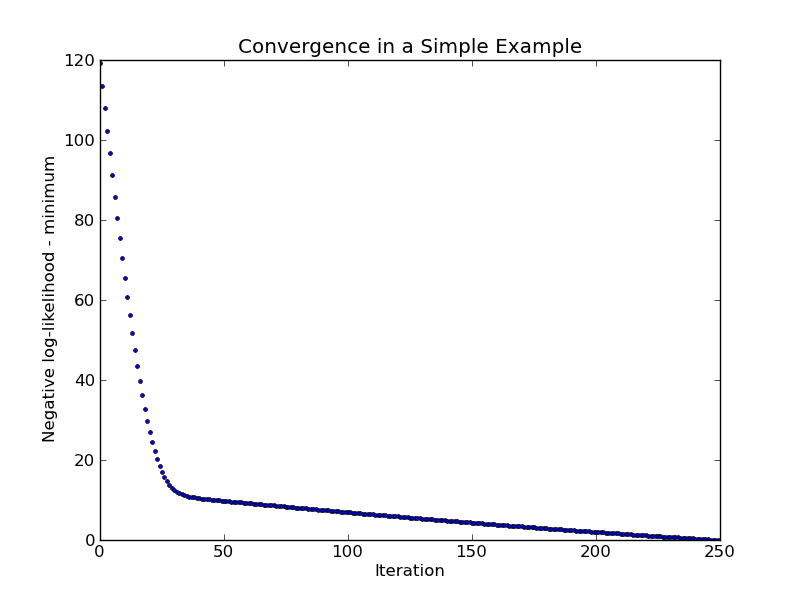
\includegraphics[width=8in]{likelihood.png}
%\end{figure}
%\end{block}


%\begin{block}{Comparison with Other Methods}

To test convergence, we applied 100 different random rigid transformations to the test data and used both ICP and GP to recover the transformation parameters. We then recorded the mean-squared error (MSE) between the original and transformed scene.

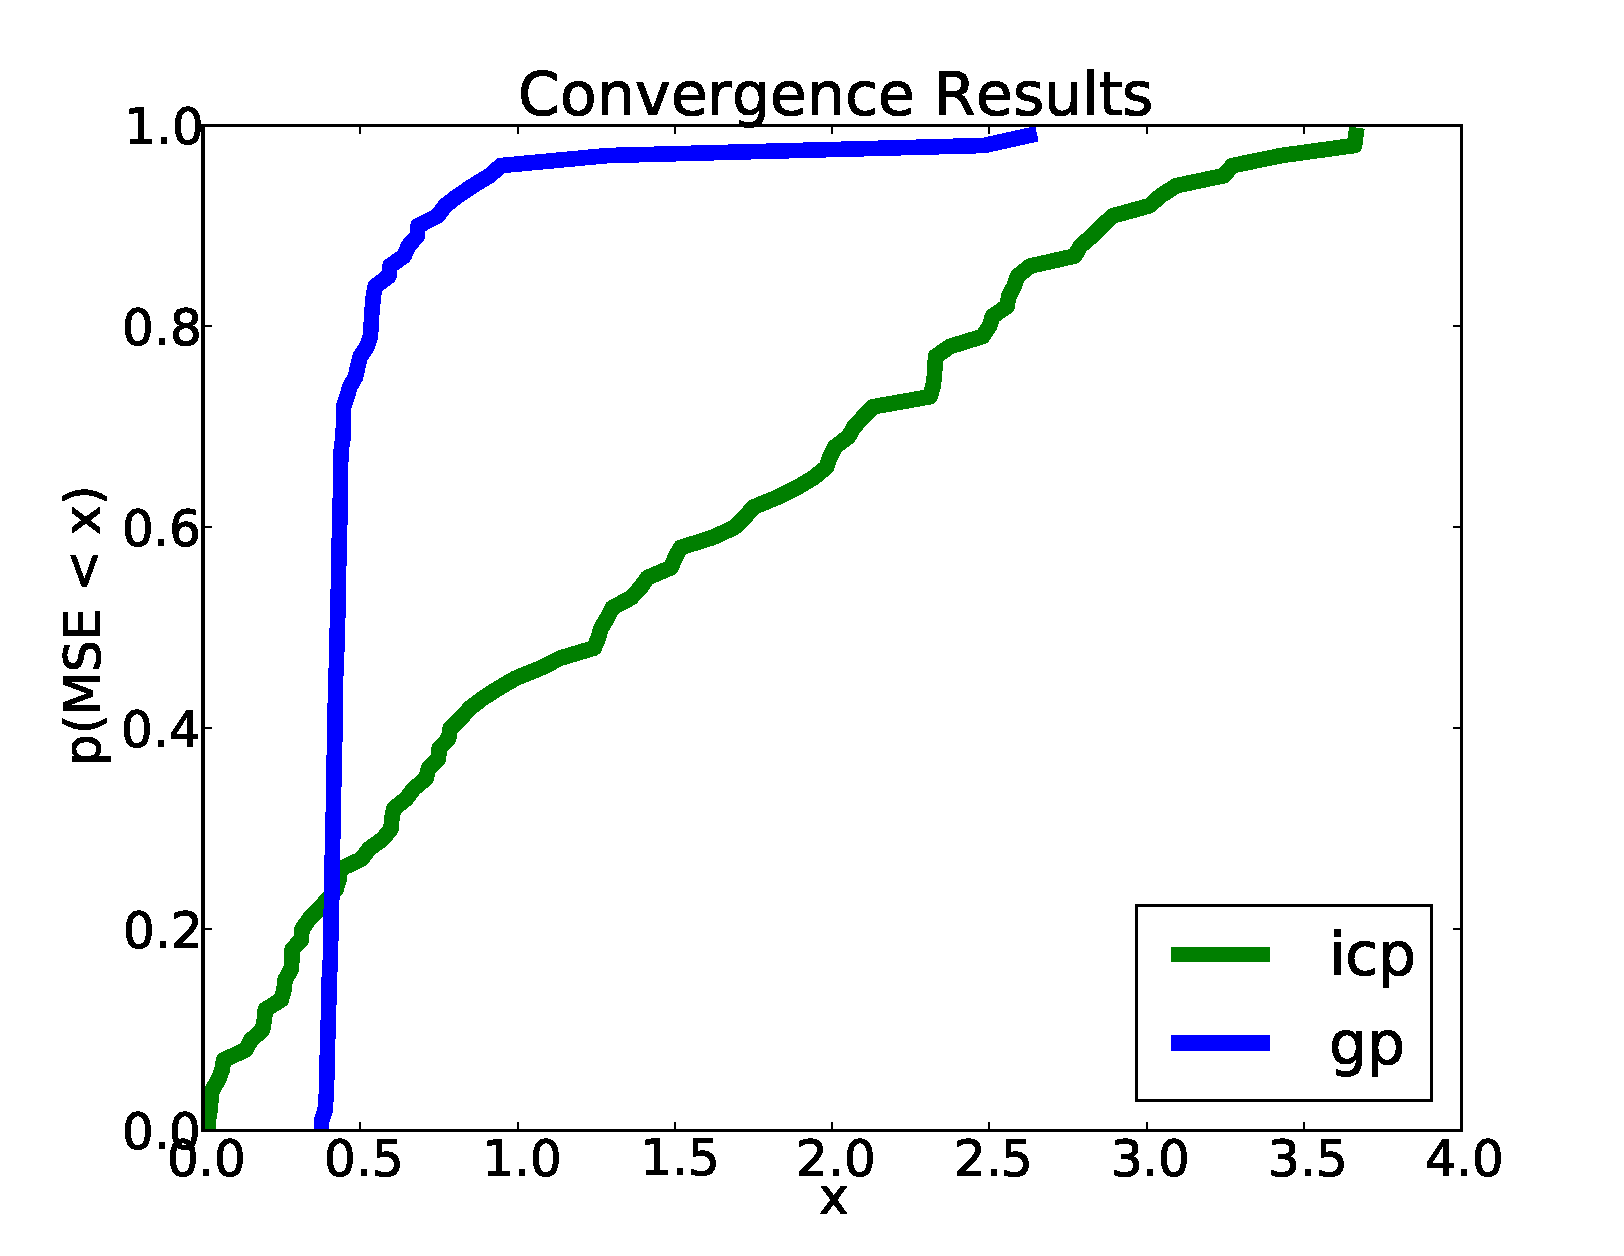
\includegraphics[width=10in]{convergence2.pdf}

CDF of MSE values. Our method on average provides better convergence than ICP.

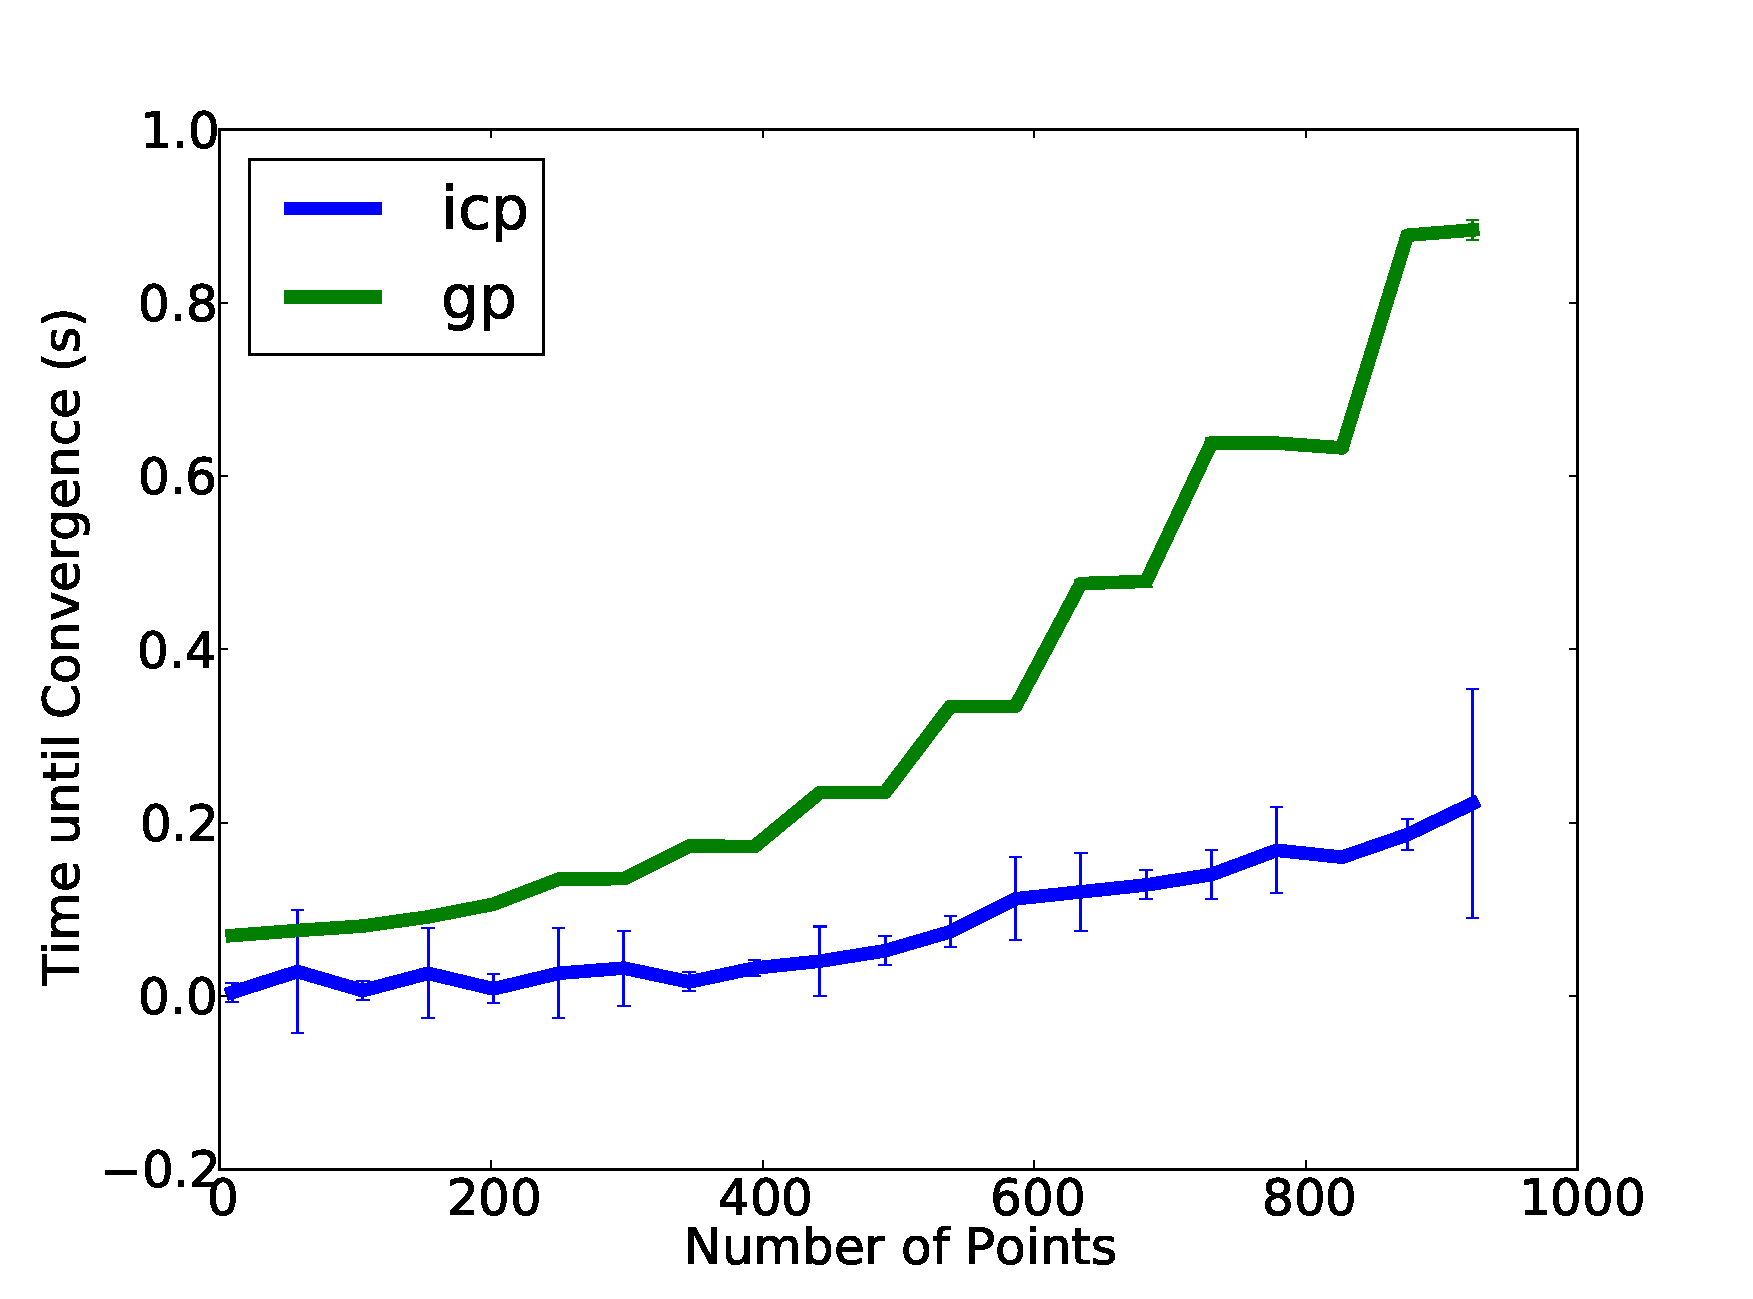
\includegraphics[width=10in]{scaling2.pdf}
\end{block}

Scaling as the number of points in the cloud increase. Our method adds a minimal amount of overhead over ICP.

\begin{block}{Conclusions}
\begin{itemize}
\item Gaussian Processes can represent and recover the transformation of a 3D scene
\item The convergence rate and speed of Gaussian Processes outperforms ICP
\item Robustness still needs work: much better performance with small transformations
\item Needs to be evaluated with real point cloud data
\item Currently only handles elevation data: general 3D point clouds require modeling density
\item Newton's method is a straightforward extension, given derivation of Hessian
\end{itemize}
\end{block}


\end{textblock}

\end{frame}
\end{document}
